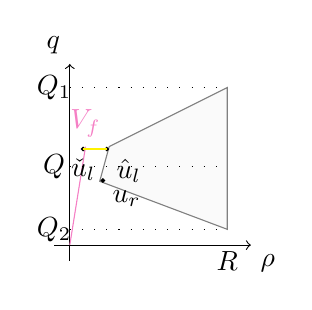
\begin{tikzpicture}
% coordinates
    \filldraw[fill=black!2, draw=black!50] plot [tension = 1] coordinates { (0.5,1.25) (2,2) (2,0.2) (0.38, 0.81) (0.5,1.25)};
    \draw[->] (0,-0.2) -- (0,2.3) node[anchor=south east] {$q$};
   
    \draw[magenta!50] (0,0) -- (0.2,1.25) node[anchor = south] {$V_f$};
    
    \filldraw[black] (0.42,0.82) circle (0.6pt) node[anchor = north west]{$u_r$} ;
    \filldraw[black] (0.47,1.22) circle (0.6pt) node[anchor = north west]{$\hat u_l$} ;
    \filldraw[black] (0.17,1.22) circle (0.6pt) node[anchor = north]{$\check u_l$} ;
    % \node at (1,1) {$\Omega_c$};
     \draw[->] (-0.2,0) -- (2.3,0) node[anchor=north west] {$\rho$};
    % contact disk
    \draw[line width=0.45mm, orange!50, domain=0.35:0.47]  plot[id=x] function{(x/0.47)*(2-0.47)/(2-x)*1.2};
    % \draw[-][black!50] (0, 0.98) -- (2, 0.2) node[anchor=south west] {$q_m(\rho)$} ;
    \node at (2,-0.2) {$R$};
     \node at (-0.2,2) {$Q_1$};
     \node at (-0.2,0.2) {$Q_2$};
     \node at (-0.2,1) {$Q$};
     \draw[loosely dotted] (0,1) -- (2,1);
     \draw[loosely dotted] (0,2) -- (2,2);
     \draw[loosely dotted] (0,0.2) -- (2,0.2);
     %\node at (1.2,-0.5) {$(3a)$};
     % rarefactions and shocks
    %\draw[lime] (1.05, 1.33) -- (2, 1.6) ;
    %\draw[<-][cyan!50] (0.42, 1.19) -- (1, 1.33) ;
    
    %\draw[->][lime] (1.48,0.4)  -- (2, 0.2) ;
    \draw[line width=0.35mm, yellow] (0.17,1.22) -- (0.47,1.22) ;
     
\end{tikzpicture}